% Options for packages loaded elsewhere
\PassOptionsToPackage{unicode}{hyperref}
\PassOptionsToPackage{hyphens}{url}
\documentclass[12pt, ]{article}

\usepackage{mathtools}
\usepackage{amsmath}
\usepackage{amsthm}
\usepackage{amssymb}
\usepackage[italicdiff]{physics}
\mathtoolsset{showonlyrefs}

% SPACING AND FONTS %%%%%%%%%%%%%%%%%%%%%%%%%%%%%%%%%%%%%%%%%%%%%%%%%%%%%%%%%%%%
\usepackage{iftex}
% CAREFUL: the order of font includes here is very important!
\ifPDFTeX
  \usepackage[OT1,T1]{fontenc}
  \usepackage[utf8]{inputenc}
  \usepackage{textcomp} % provide euro and other symbols
    \usepackage[p,osf,swashQ]{cochineal}
  \usepackage[cochineal,vvarbb]{newtxmath}
      \usepackage[scale=0.95]{biolinum}
    \usepackage[scale=0.95,varl]{inconsolata}
\else % if luatex or xetex
  \usepackage[scale=0.95,varl]{inconsolata}
  \usepackage{newpxtext}
  \usepackage{mathpazo}
    \usepackage[scale=0.95]{biolinum}
  \fi
\ifLuaTeX
  \usepackage{selnolig}  % disable illegal ligatures
\fi
\IfFileExists{microtype.sty}{% use microtype if available
  \usepackage[]{microtype}
  \UseMicrotypeSet[protrusion]{basicmath} % disable protrusion for tt fonts
}{}

\setlength{\parindent}{0pt}
\setlength{\parskip}{10pt plus 2pt minus 2pt}
\setlength{\emergencystretch}{3em} % prevent overfull lines
\widowpenalty=10000
\clubpenalty=10000
\flushbottom
\allowdisplaybreaks
\sloppy


% CORE PACKAGES %%%%%%%%%%%%%%%%%%%%%%%%%%%%%%%%%%%%%%%%%%%%%%%%%%%%%%%%%%%%
\usepackage[dvipsnames,svgnames,x11names]{xcolor}
\usepackage[lmargin=1.5in,rmargin=1.5in,tmargin=1.08in,bmargin=1.1in]{geometry}
\usepackage[format=plain,
  labelfont={bf,sf,small,singlespacing},
  textfont={sf,small,singlespacing},
  justification=justified,
  margin=0.25in]{caption}

% SECTIONS AND HEADINGS %%%%%%%%%%%%%%%%%%%%%%%%%%%%%%%%%%%%%%%%%%%%%%%%%%%%%%%%
\setcounter{secnumdepth}{4}
\usepackage{sectsty}
\usepackage[compact]{titlesec}
% short title
\makeatletter
\newcommand\@shorttitle{}
\newcommand\shorttitle[1]{\renewcommand\@shorttitle{#1}}
\usepackage{fancyhdr}
\fancyhf{}
\pagestyle{fancy}
\renewcommand{\headrulewidth}{0pt}
\fancyheadoffset{0pt}
%\lhead{\scshape \@shorttitle}
%\rhead{\scshape\today}
\cfoot{\thepage}
\makeatother
% abstract styling
\renewenvironment{abstract}{
  \centerline
  {\large\sffamily\bfseries Abstract}\vspace{-1em}
  \begin{quote}\small
}{
  \end{quote}
}

% PANDOC INCLUDES %%%%%%%%%%%%%%%%%%%%%%%%%%%%%%%%%%%%%%%%%%%%%%%%%%%%%%%%%%%%%%

\providecommand{\tightlist}{%
  \setlength{\itemsep}{0pt}\setlength{\parskip}{0pt}}\usepackage{longtable,booktabs,array}
\usepackage{calc} % for calculating minipage widths
% Correct order of tables after \paragraph or \subparagraph
\usepackage{etoolbox}
\makeatletter
\patchcmd\longtable{\par}{\if@noskipsec\mbox{}\fi\par}{}{}
\makeatother
% Allow footnotes in longtable head/foot
\IfFileExists{footnotehyper.sty}{\usepackage{footnotehyper}}{\usepackage{footnote}}
\makesavenoteenv{longtable}
\usepackage{graphicx}
\makeatletter
\def\maxwidth{\ifdim\Gin@nat@width>\linewidth\linewidth\else\Gin@nat@width\fi}
\def\maxheight{\ifdim\Gin@nat@height>\textheight\textheight\else\Gin@nat@height\fi}
\makeatother
% Scale images if necessary, so that they will not overflow the page
% margins by default, and it is still possible to overwrite the defaults
% using explicit options in \includegraphics[width, height, ...]{}
\setkeys{Gin}{width=\maxwidth,height=\maxheight,keepaspectratio}
% Set default figure placement to htbp
\makeatletter
\def\fps@figure{htbp}
\makeatother
% END PANDOC %%%%%%%%%%%%%%%%%%%%%%%%%%%%%%%%%%%%%%%%%%%%%%%%%%%%%%%%%%%%%%%%%%%

% USER INCLUDES %%%%%%%%%%%%%%%%%%%%%%%%%%%%%%%%%%%%%%%%%%%%%%%%%%%%%%%%%%%%%%%%
% additional LaTeX code for the "preamble" goes here
\makeatletter
\makeatother
\makeatletter
\makeatother
\makeatletter
\@ifpackageloaded{caption}{}{\usepackage{caption}}
\AtBeginDocument{%
\ifdefined\contentsname
  \renewcommand*\contentsname{Table of contents}
\else
  \newcommand\contentsname{Table of contents}
\fi
\ifdefined\listfigurename
  \renewcommand*\listfigurename{List of Figures}
\else
  \newcommand\listfigurename{List of Figures}
\fi
\ifdefined\listtablename
  \renewcommand*\listtablename{List of Tables}
\else
  \newcommand\listtablename{List of Tables}
\fi
\ifdefined\figurename
  \renewcommand*\figurename{Figure}
\else
  \newcommand\figurename{Figure}
\fi
\ifdefined\tablename
  \renewcommand*\tablename{Table}
\else
  \newcommand\tablename{Table}
\fi
}
\@ifpackageloaded{float}{}{\usepackage{float}}
\floatstyle{ruled}
\@ifundefined{c@chapter}{\newfloat{codelisting}{h}{lop}}{\newfloat{codelisting}{h}{lop}[chapter]}
\floatname{codelisting}{Listing}
\newcommand*\listoflistings{\listof{codelisting}{List of Listings}}
\makeatother
\makeatletter
\@ifpackageloaded{caption}{}{\usepackage{caption}}
\@ifpackageloaded{subcaption}{}{\usepackage{subcaption}}
\makeatother
\makeatletter
\@ifpackageloaded{tcolorbox}{}{\usepackage[skins,breakable]{tcolorbox}}
\makeatother
\makeatletter
\@ifundefined{shadecolor}{\definecolor{shadecolor}{rgb}{.97, .97, .97}}
\makeatother
\makeatletter
\makeatother
\makeatletter
\makeatother
% END USER INCLUDES %%%%%%%%%%%%%%%%%%%%%%%%%%%%%%%%%%%%%%%%%%%%%%%%%%%%%%%%%%%%

% BIBLIOGRAPHY %%%%%%%%%%%%%%%%%%%%%%%%%%%%%%%%%%%%%%%%%%%%%%%%%%%%%%%%%%%%%%%%%
\usepackage[]{natbib}
\bibliographystyle{apalike}

% Give it this name so that it works with ::: #refs
\newenvironment{CSLReferences}[2]{
\bibliography{aqrd-final-refs.bib}
\clearpage
}{}

% LINKS %%%%%%%%%%%%%%%%%%%%%%%%%%%%%%%%%%%%%%%%%%%%%%%%%%%%%%%%%%%%%%%%%%%%%%%%
\usepackage{hyperref}
\usepackage{url}
\hypersetup{
  pdftitle={A Further Exploration of Disparate Racial Exposure to Particulate Matter in Light of Covid-19 Shutdowns},
  pdfauthor={Andre Eanes},
  colorlinks=true,
  linkcolor={black},
  filecolor={Maroon},
  citecolor={VioletRed4},
  urlcolor={DodgerBlue4},
  pdfcreator={LaTeX via pandoc}}

% TITLE, AUTHOR, DATE %%%%%%%%%%%%%%%%%%%%%%%%%%%%%%%%%%%%%%%%%%%%%%%%%%%%%%%%%%
\title{\sffamily\bfseries\huge\parfillskip=0pt
\rightskip=0pt plus .5\textwidth
\leftskip=0pt plus .5\textwidth
\emergencystretch=.3\textwidth A Further Exploration of Disparate Racial
Exposure to Particulate Matter in Light of Covid-19 Shutdowns}
\shorttitle{A Further Exploration of Disparate Racial Exposure to Particulate Matter in Light of Covid-19 Shutdowns}
\author{\textbf{Andre Eanes}
 }
\date{}


\begin{document}
\allsectionsfont{\sffamily}

\maketitle

\begin{abstract}
In 2020, the onset of the Covid-19 pandemic provided a unique
opportunity to study how reduced vehicle traffic may have lowered levels
of air pollution in cities. Bluhm et al.~(2022) explored this phenomenon
throughout the state of California in light of state-wide pandemic
shutdowns to determine how different demographic groups may have
benefitted from this change. They found that the most historically
marginalized groups (Black, Hispanic/Latinx, and low-income communities)
had the highest exposure to particulate matter (PM2.5) and nitrous
oxides (NOx) prior to Covid-19 as the baseline scenario, and while their
exposure was still among the highest during the Covid-19 shutdown period
in 2020, the absolute difference in exposure to air pollution between
groups was reduced. I built on these findings to further investigate
this relationship with PM2.5 among highly segregated vs.~more diverse
communities, also finding a reduction PM2.5 exposure across groups,
although the largest reductions were seen Black and some Hispanic/Latinx
communities. I also analyzed how PM2.5 differed overall between years by
county, which yielded mixed results but overall a small (9.9\%)
reduction in average PM2.5 concentrations when weighted by sensor data
availability and how well it represents the county-level population. In
addition, this study highlights the importance of using a diverse set of
fixed effects, as was the case with Bluhm et al.~(2022), to further
study what factors may contribute to and confound an understanding of
air pollution exposure.
\end{abstract}

\ifdefined\Shaded\renewenvironment{Shaded}{\begin{tcolorbox}[frame hidden, borderline west={3pt}{0pt}{shadecolor}, breakable, interior hidden, sharp corners, boxrule=0pt, enhanced]}{\end{tcolorbox}}\fi



% USER BODY %%%%%%%%%%%%%%%%%%%%%%%%%%%%%%%%%%%%%%%%%%%%%%%%%%%%%%%%%%%%%%%%%%%%

\hypertarget{introduction}{%
\section{Introduction}\label{introduction}}

Issues of health and equity related to air quality, particularly in
urban contexts, have gained increasing attention in recent years along
with the emergence of interdisciplinary environmental justice
scholarship. The onset of the Covid-19 pandemic, however, provided an
incredibly unique set of conditions to study how patterns of urban air
pollution change in response to a sudden decrease in vehicle emissions,
as well as how other contributors to air pollution may or may not follow
this trend. \citet{bluhm_disparate_2022}, the focus of this paper whose
findings I extend, explore this phenomenon in great detail through a
two-way fixed effects analysis. They study how different demographic
groups may be disproportionately impacted by air pollution, what
confounding spatial and temporal variables can be accounted for in order
to more accurately study such impacts, and the effects on this
relationship as a result of the Covid-19 shutdown after stay-at-home
orders were fully in place throughout the state of California between
late March and April of 2020.

While numerous, one major finding of this study reinforced an
increasingly well-understood theme in environmental justice, but with an
insightful twist in light of Covid-19. This is that low-income and
racially marginalized groups already experienced disproportionately high
levels of air pollution - in this case, particulate matter (PM2.5) and
nitrogen oxides (NOx) - in baseline conditions prior to Covid-19, but as
a result of emissions decreasing universally in most places, the level
of disparity between groups in terms of the absolute concentration of
pollutants decreased. While overarching differences in harmful pollution
between more affluent communities and their low-income counterparts
remained even during the Covid-19 shutdown (i.e., there was little
change in terms of the ordinal relationship between groups), the
historically worst-affected communities experienced a notable
improvement in their exposure to PM2.5 and NOx.
\citet{camilleri_air_2023} analyze a similar case in Chicago, albeit in
a more predictive capacity, finding that the electrification of
heavy-duty vehicles would most likely provide the greatest health
benefits to Black and Hispanic/Latinx communities through a relatively
larger reduction in exposure to air pollution.
\citet{bluhm_disparate_2022} visualize this phenomenon in terms of the
actual underlying patterns of changes in the frequency of driving
(``mobility'') and through a theoretical representation of exposure by
demographic group in Figures 2b and ED1, respectively.

Other studies have explored various aspects of the dynamics between
race, class, income, and health outcomes related to air pollution, both
regarding baseline conditions Covid-19 notwithstanding as well as the
specific ramifications of pandemic lock-downs.
\citet{mikati_disparities_2018} and \citet{mohai_racial_2009} serve as
prominent examples demonstrating disproportionate proximity of emissions
sources and overall exposure to hazardous air pollutants among racial
minorities, particularly ones which are predominantly Black and
Hispanic/Latinx, as well as low-income communities.
\citet{mikati_disparities_2018} used a national point-source emissions
database combined with American Community Survey (ACS) data to determine
particulate matter exposure among racial groups and poverty thresholds,
while both studies analyzed siting patterns of hazardous industrial
facilities in relation to numerous factors, notably race, gender, age,
and urban vs.~rural residence. In addition to the aforementioned groups,
\citet{mohai_racial_2009} found heightened likelihood of exposure to
hazardous sources of emissions among those closer to cities, living in
the South or Northeast, with low educational attainment, and over the
age of 65. In the context of Covid-19, \citet{bekbulat_changes_2021} and
\citet{ali_exposure_2021}, respectively, present additional evidence
that most pollutants notably decreased in their concentration during the
Covid-19 shutdown periods (albeit with different trends and delays), and
that exposure to high concentration of particulate matter can lead to
more severe Covid-19 symptoms.

\citet{bluhm_disparate_2022} use highly complex models to fix for
weather, transportation, and infrastructural components over space and
time, as well as accounting for various racial and economic
characteristics. Doing so served to both isolate the relationship with
air pollution exposure among variables of interest (mostly demographic),
as well as to reduce the influence of exogenous confounding variables.
Given this complexity, accurately replicating and analyzing all fixed
effects would be beyond the scope of this paper, thus requiring a
narrower and/or fuzzier analysis of major variables. To differentiate
from and extend upon Bluhm et al.'s findings, I have conducted a series
of analyses on particulate matter exposure which narrow in on the exact
period during which Covid-19 lock-down was fully implemented in
California (March 20th - April 30th), along with the same dates in 2019,
to elucidate a relationship between race and PM2.5 exposure. Isolating
this period of relatively uniform mobility trends during the onset of
Covid-19, along with a selection of days within a narrow seasonal range,
effectively serves as a time fixed effect. Given this narrower period
within each year, I provide further analysis and insight regarding the
variance in particulate matter exposure among more racially segregated
versus more diverse communities as well as the county-level trends in
air pollution between years, also highlighting the challenges associated
with identifying appropriate and usable temporal and geographic
delineations for analysis. While all analyses were constrained to March
and April of each year, geographic groupings vary between the sensor
level, Census block group, county level, and state level depending on
the granularity and scope required for each result.

In analyzing exposure among communities of different racial
compositions, I grouped sensor particulate matter readings by year and a
racial designation category associated with whether or not a particular
racial group dominated each Census block, represented through
Figure~\ref{fig-dp} in marginal density plots form. Figure~\ref{fig-rd}
and Figure~\ref{fig-bi} show county-level PM2.5 exposure using a
weighting convention based on the availability and robustness of sensor
data within each county. I find that overall year-over-year changes in
PM2.5 exposure were mixed, partly as a result of the chosen geographic
delineations and the fuzzy nature of the analysis. However, PM2.5 was
reduced on average between March-April 2019 and 2020, exhibited clear
discrepancies between racial groups, and showed fewer high readings
uniformly across groups, with an exception among Hispanic/Latinx
populations, whose exposure assumed a bimodal distribution in 2020, with
some areas showing lower PM2.5 concentrations and others showing higher
exposure, likely as a result of shifting emissions patterns. This
analysis highlights the clear differences in exposure among racial
groups as well as the importance of incorporating fixed effects where
possible to show the varied drivers of urban air pollution (including
and beyond vehicle traffic) to more accurately parse out
environmental-justice-critical air pollution exposure among low-income
and minority racial groups, particularly given the numerous changes
which can occur around a large-scale shock such as Covid-19 shutdowns.

\hypertarget{data-methods}{%
\section{Data \& Methods}\label{data-methods}}

The key variables used in this and the original study are summarized in
Figure~\ref{fig-sumtable}, notably particulate matter readings, Census
block-level population and racial composition, and median income. Except
for PM2.5, the remaining variables were virtually unchanged between the
studied periods in 2019 and 2020. All variables are derived from
individual data points on the sensor- and daily-observation-level,
except for county-level PM2.5 averages, which are derived from the same
sensor-observation-level data but are summarized based on 56 observed
counties and each year.

\begin{figure}[H]

{\centering 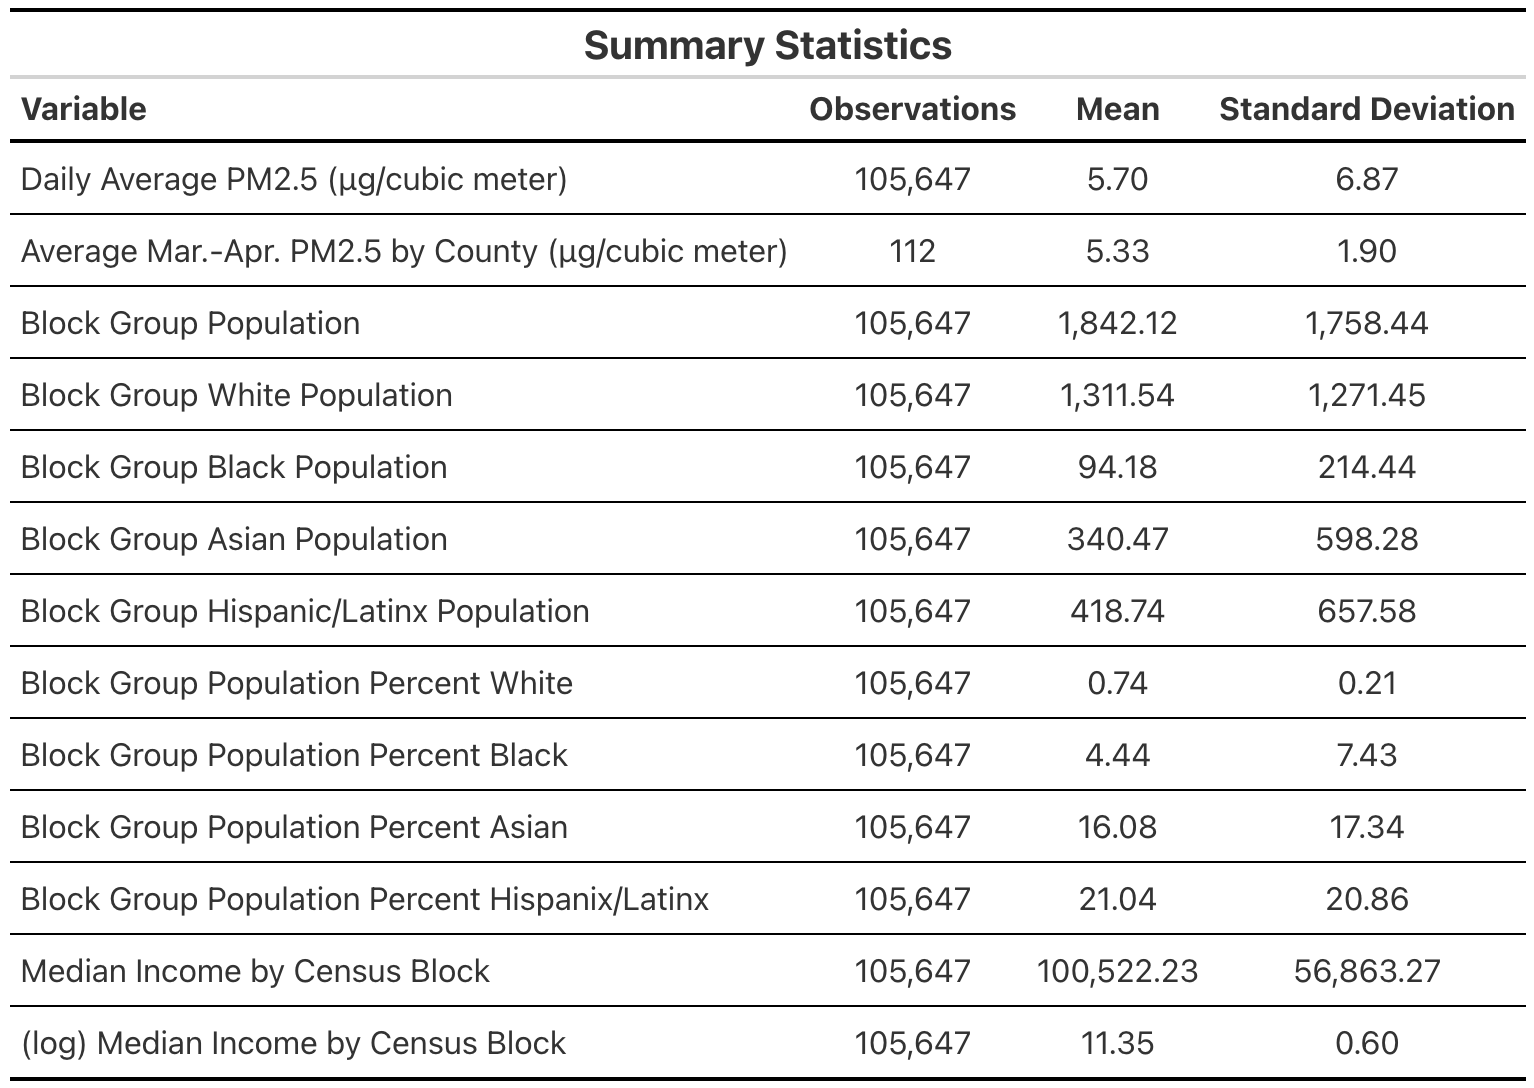
\includegraphics{figures/PM_SumStatsTable.png}

}

\caption{\label{fig-sumtable}Table of summary statistics, including
daily and annual particulate matter (PM2.5) readings, block group
populations in total and by race, compositions of various racial groups
in each block group, and median income (as well as a log of income for
linear comparison with PM2.5) by block group.}

\end{figure}

The underlying data for this analysis were a combination of Census
Bureau demographic data and particulate matter concentration data (PM2.5
µg/cubic meter), the latter of which were gathered from California Air
Resources Board (CARB) professional-grade air monitors and PurpleAir
units (low-cost sensors often used in domestic or educational settings).
Code in the original replication package from
\citet{bluhm_disparate_2022} joins these to capture all key variables,
and then creates two datasets which were directly used in this analysis,
one of which lists one row per daily sensor observation (denoted as the
``wide'' dataset), the other of which duplicates each daily sensor
observation row once for each key demographic characteristic by block
(log median income, percent Black, and percent Asian, and percent
Hispanic/Latinx), creating a long format dataset four times the length
as the first.

I first grouped the wide data by county and year and then weighted each
sensor based on the completeness of its data relative to other sensors,
finally weighting counties (assigned values between 0 and 1) based on
the sensor readings in each relative to the total population of the
corresponding county. I then plotted these values in a
pseudo-regression-discontinuity format with the weight as the running
variable and average county-level PM2.5 concentrations during each
March-April annual period as show in Figure~\ref{fig-rd} (weights for
2020 are flipped and put between 1 and 2 such that 1 is the cutoff
between years). I then took the same data and plotted them simply by
year without weights as the running variable to have a simpler binary
representation of any year-over-year differences. Note that the use of
weights as the running variable in this format is not conducive to a
beset fit line - rather, differences are highlighted with horizontal
dotted lines at the weighted mean for each year.

To create Figure~\ref{fig-dp}, I took daily-sensor-observation-level
data, this time using the long format dataset, and assigned a
categorical dummy variable to whether each observation is in a Census
block with a majority or vast majority of a given racial group, or if no
groups exceed 50\% (thus, all bins are mutually exclusive and
collectively exhaustive). With these delineations, I grouped the
observations in blocks with no group exceeding 50\% (``Relatively
Diverse'') along with those with a group exceeding 50\% but not 80\%
(``Majority\ldots{}''), and then I grouped only blocks comprised of
greater than 80\% of a single racial group (``Vast Majority\ldots{}'').
I took these groups, also separated by year, and plotted them as a
marginal density plot.

Finally, I grouped the long format dataset by year and demogrpahic
group, running linear regressions for each subset between PM2.5
concentration and percent composition of the chosen demographic. The
estimating equation underlying the linear regression models summarized
in Figure~\ref{fig-reg-table} is composed as follows:
\[E_{it} = P_{is,td} + R_{ib,t}\] where \(E_{it}\) is the mean PM2.5
exposure among racial groups by each location fixed effect, categorized
under denotation \(_{i}\), during the late March to April period fixed
effect in each year, categorized under denotation \(_{t}\).
\(P_{is,td}\) represents the mean among PM2.5 concentrations on the
daily level within each each March-April annual period, denoted as
\(_{td}\), at each sensor-level location, denoted as \(_{is}\).
\(R_{ib,t}\) represents the proportion of each racial group as a percent
of the total population in each Census block, denoted as \(_{ib}\),
during each annual March-April annual period, also denoted as \(_{t}\).

\newpage

\hypertarget{results}{%
\section{Results}\label{results}}

The first set of figures plot county-level PM2.5 exposure during late
March through April of 2019 and 2020. Figure~\ref{fig-rd} uses weights
as the running variable, showing that PM2.5 did decrease consistently
year-over-year, but only slightly when represented in on the county
level and not accounting for a broader array of fixed effects.
Figure~\ref{fig-bi} shows the same county-level averages but simply as a
binary variable. Both graphs use the dotted red line to represent the
weighted mean among all counties (even Figure~\ref{fig-bi} despite not
using weighting as a running variable).

\begin{figure}[H]

{\centering 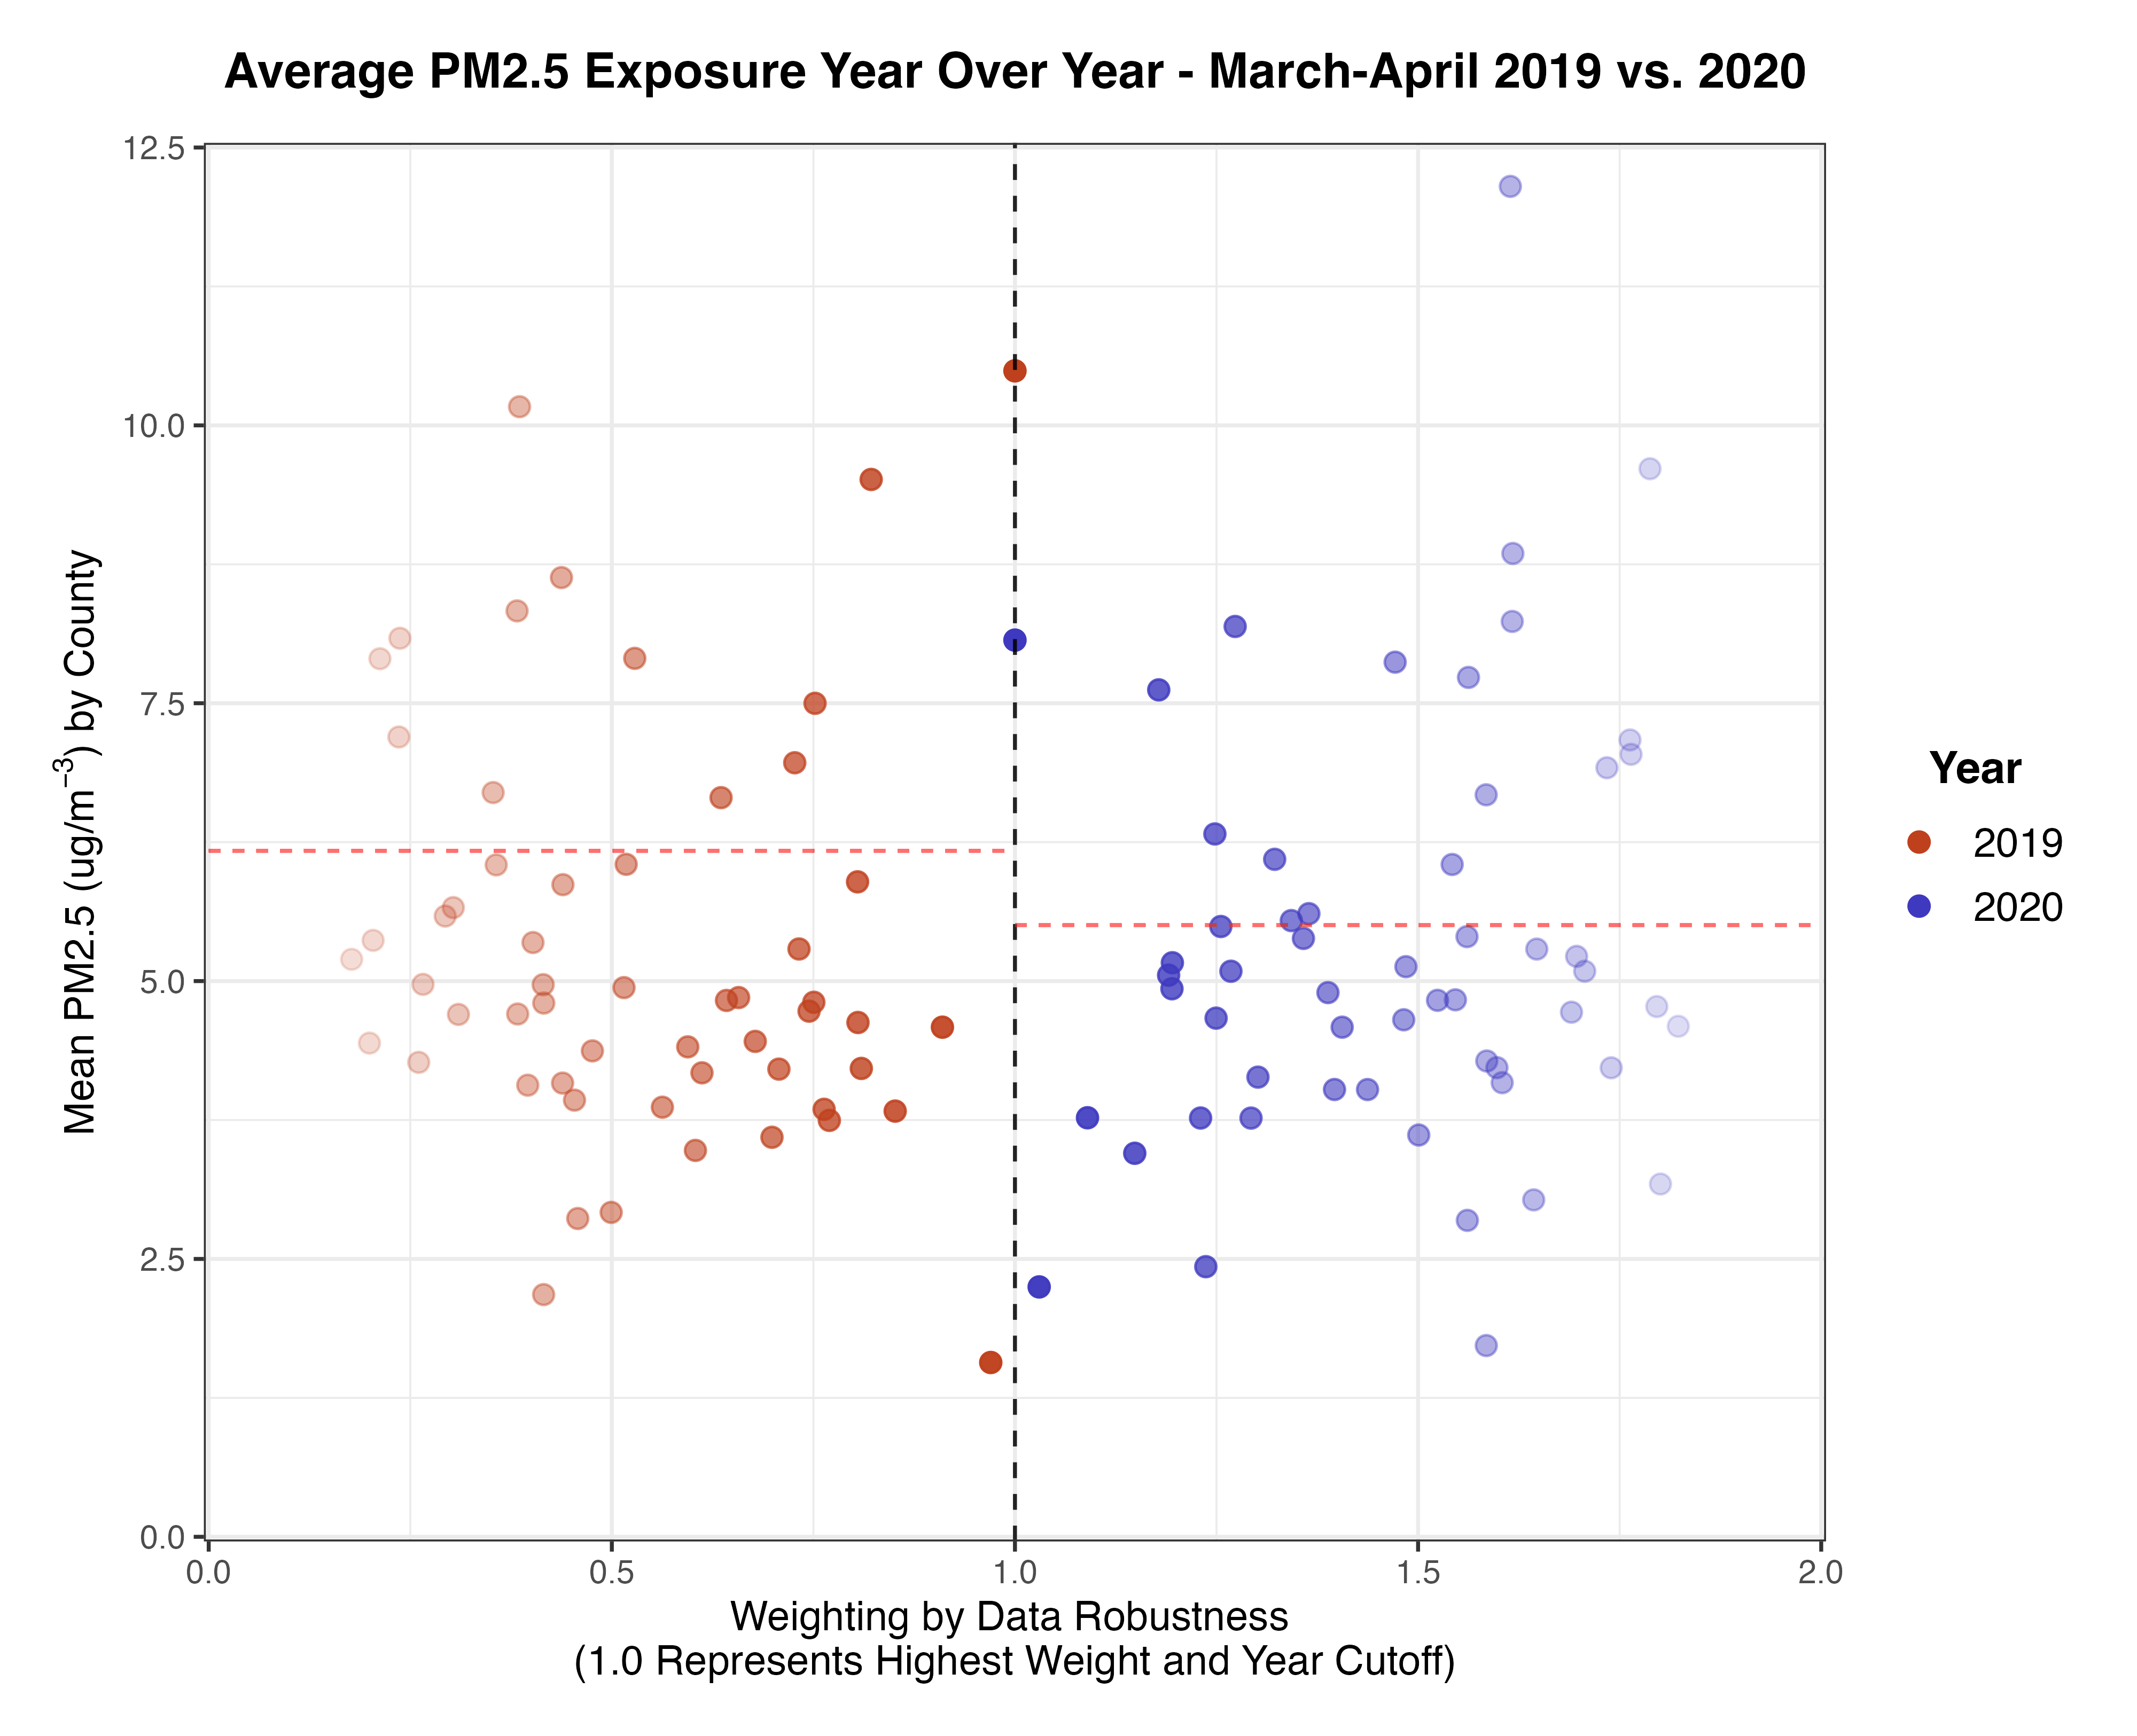
\includegraphics{figures/RD_CoWt_Scatterplot_19v20.png}

}

\caption{\label{fig-rd}Average PM2.5 concentrations by county and year,
weighed based on the overall availability and robustness of sensor data
relative to the population in each county, with points closer to 1
(higher opacity) weighted higher. Red dotted lines represent weighted
averages among counties for each year. While still exhibiting high
variance, count-level weighted mean PM2.5 was 9.9\% lower during the
2020 shutdown period than the same time in 2019.}

\end{figure}

\begin{figure}[H]

{\centering 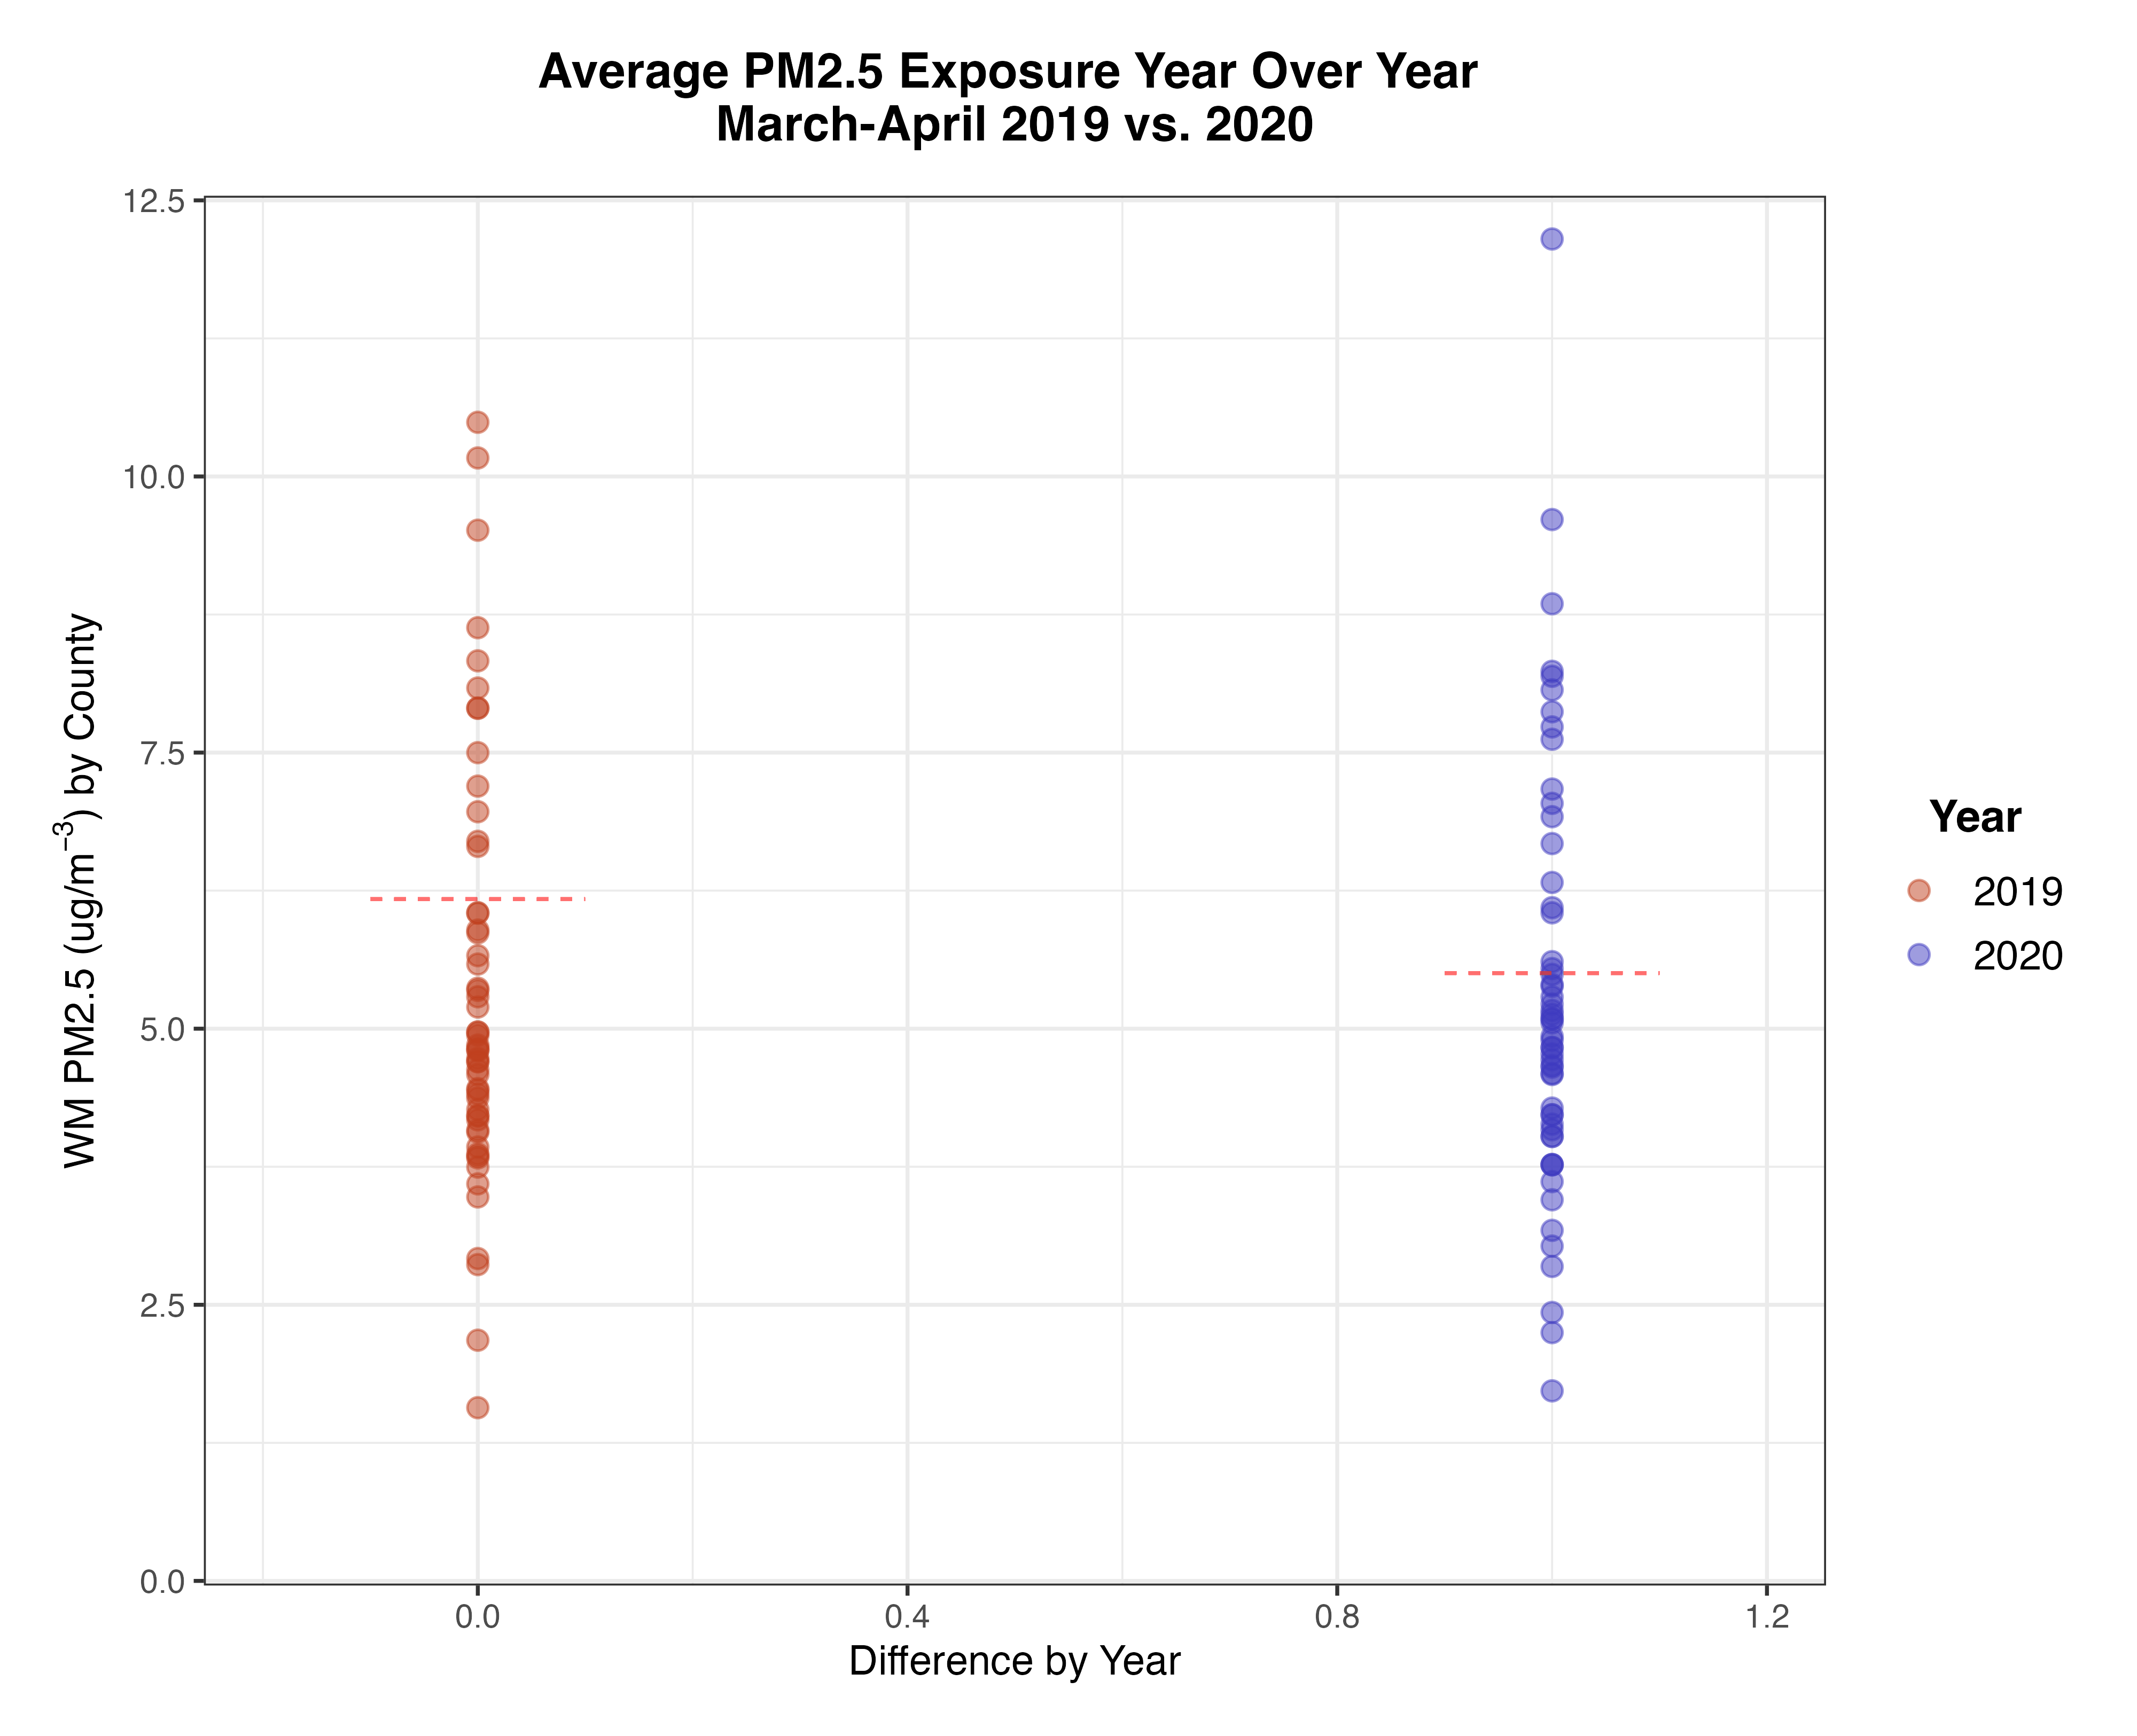
\includegraphics{figures/County_Binary_Scatterplot_19v20.png}

}

\caption{\label{fig-bi}Average PM2.5 concentrations by county and year,
with weighting and opacity assigned equally. This shows the same
distributions and weighted mean lines as Figure~\ref{fig-rd} (also a
9.9\% reduction in weighted mean PM2.5), but it visualizes each county
more evenly.}

\end{figure}

Figure~\ref{fig-dp} breaks down Census blocks by whether they exhibited
a strongly segregated racial composition and if so, by what race,
faceted by year and an upper and low racial designation category (i.e.,
highly segregated or not). Generally, predominantly Black and
Hispanic/Latinx communities experienced the highest exposure to
particulate matter in both years, although there was a noticeable shift
during the 2020 Covid-19 shutdown in which distributions became more
closely aligned among racial groups, lowering PM2.5 exposure (especially
very high concentrations values) to some degree among all groups. The
only major exception to this was a contingent of Hispanic/Latinx
communities, which actually experienced equal or higher exposure in
2020. It is possible that this is due to increased output from
electricity generation plants, which these communities may be
disproportionately sited near, or that they are already located in
highly urban settings with less of a decrease in overall pollution.

\begin{figure}[H]

{\centering 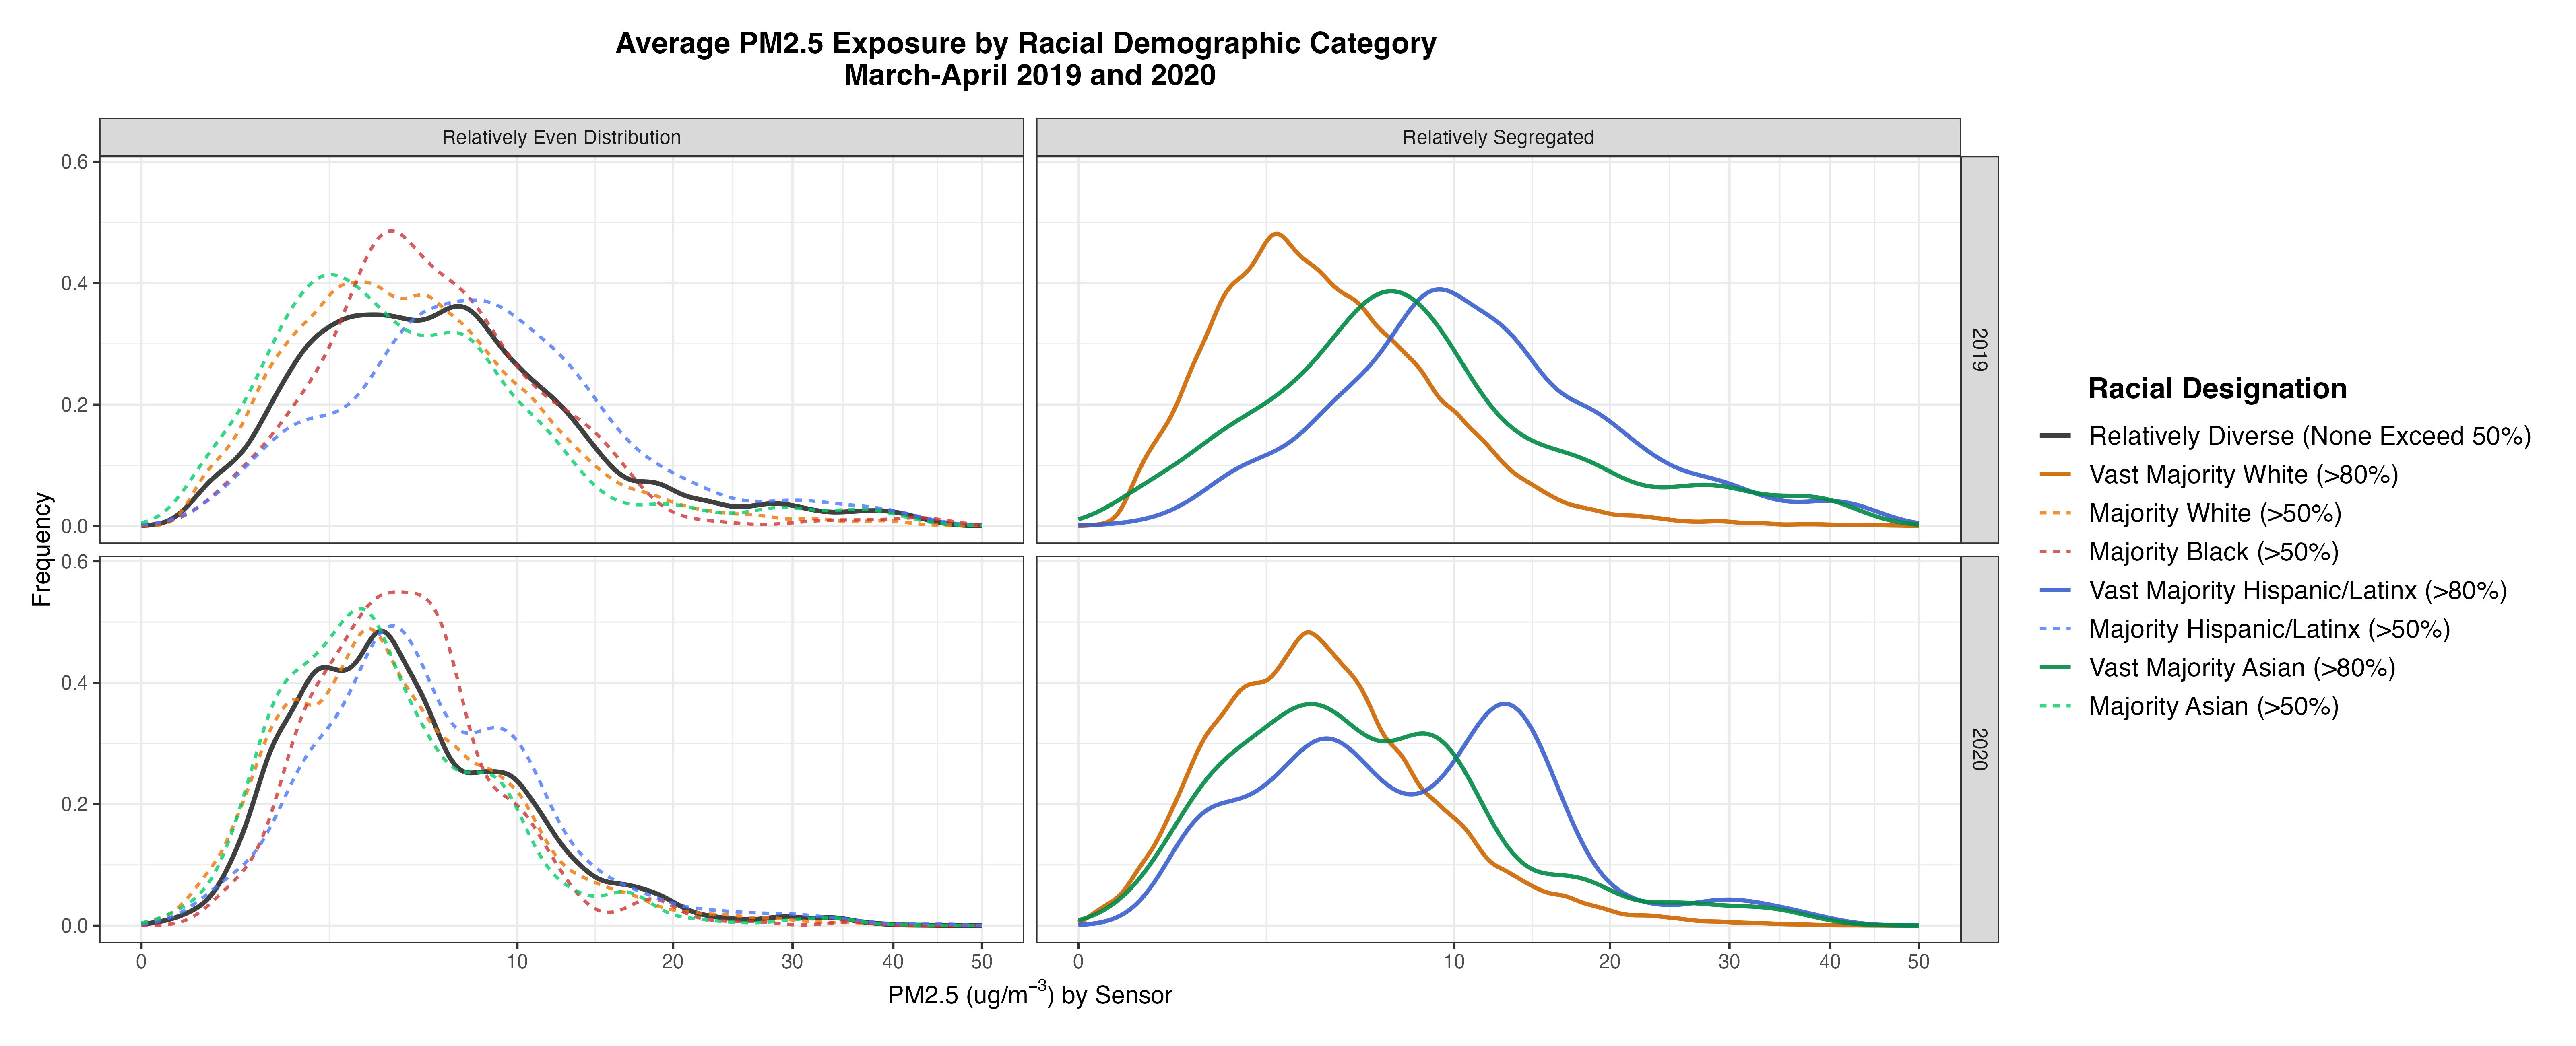
\includegraphics{figures/RaceDsgGroup_MargDensPlot_19v20+SegvDiv.png}

}

\caption{\label{fig-dp}Marginal density plot showing the distribution of
PM2.5 concentrations in late March to April 2020 based on whether each
block was relatively diverse (less than 50\% of any single racial
group), had a majority in one racial group, or had a vast majority in
one racial group (greater than 80\%). Variables are grouped by racial
designation category and faceted based on year and whether or not each
Census block had a vast majority of one group.}

\end{figure}

Finally, Figure~\ref{fig-reg-table} summarizes a series of linear
regressions conducted by year on race, income, and year.Based on these
results, low-income and predominantly Black and Hispanic/Latinx
communities have the greatest association with higher exposure to high
PM2.5 concentrations. This trend is weaker in 2020 compared to 2019, but
the overall dynamic remains relatively similar based on this fuzzy
comparison.

\begin{figure}[H]

{\centering 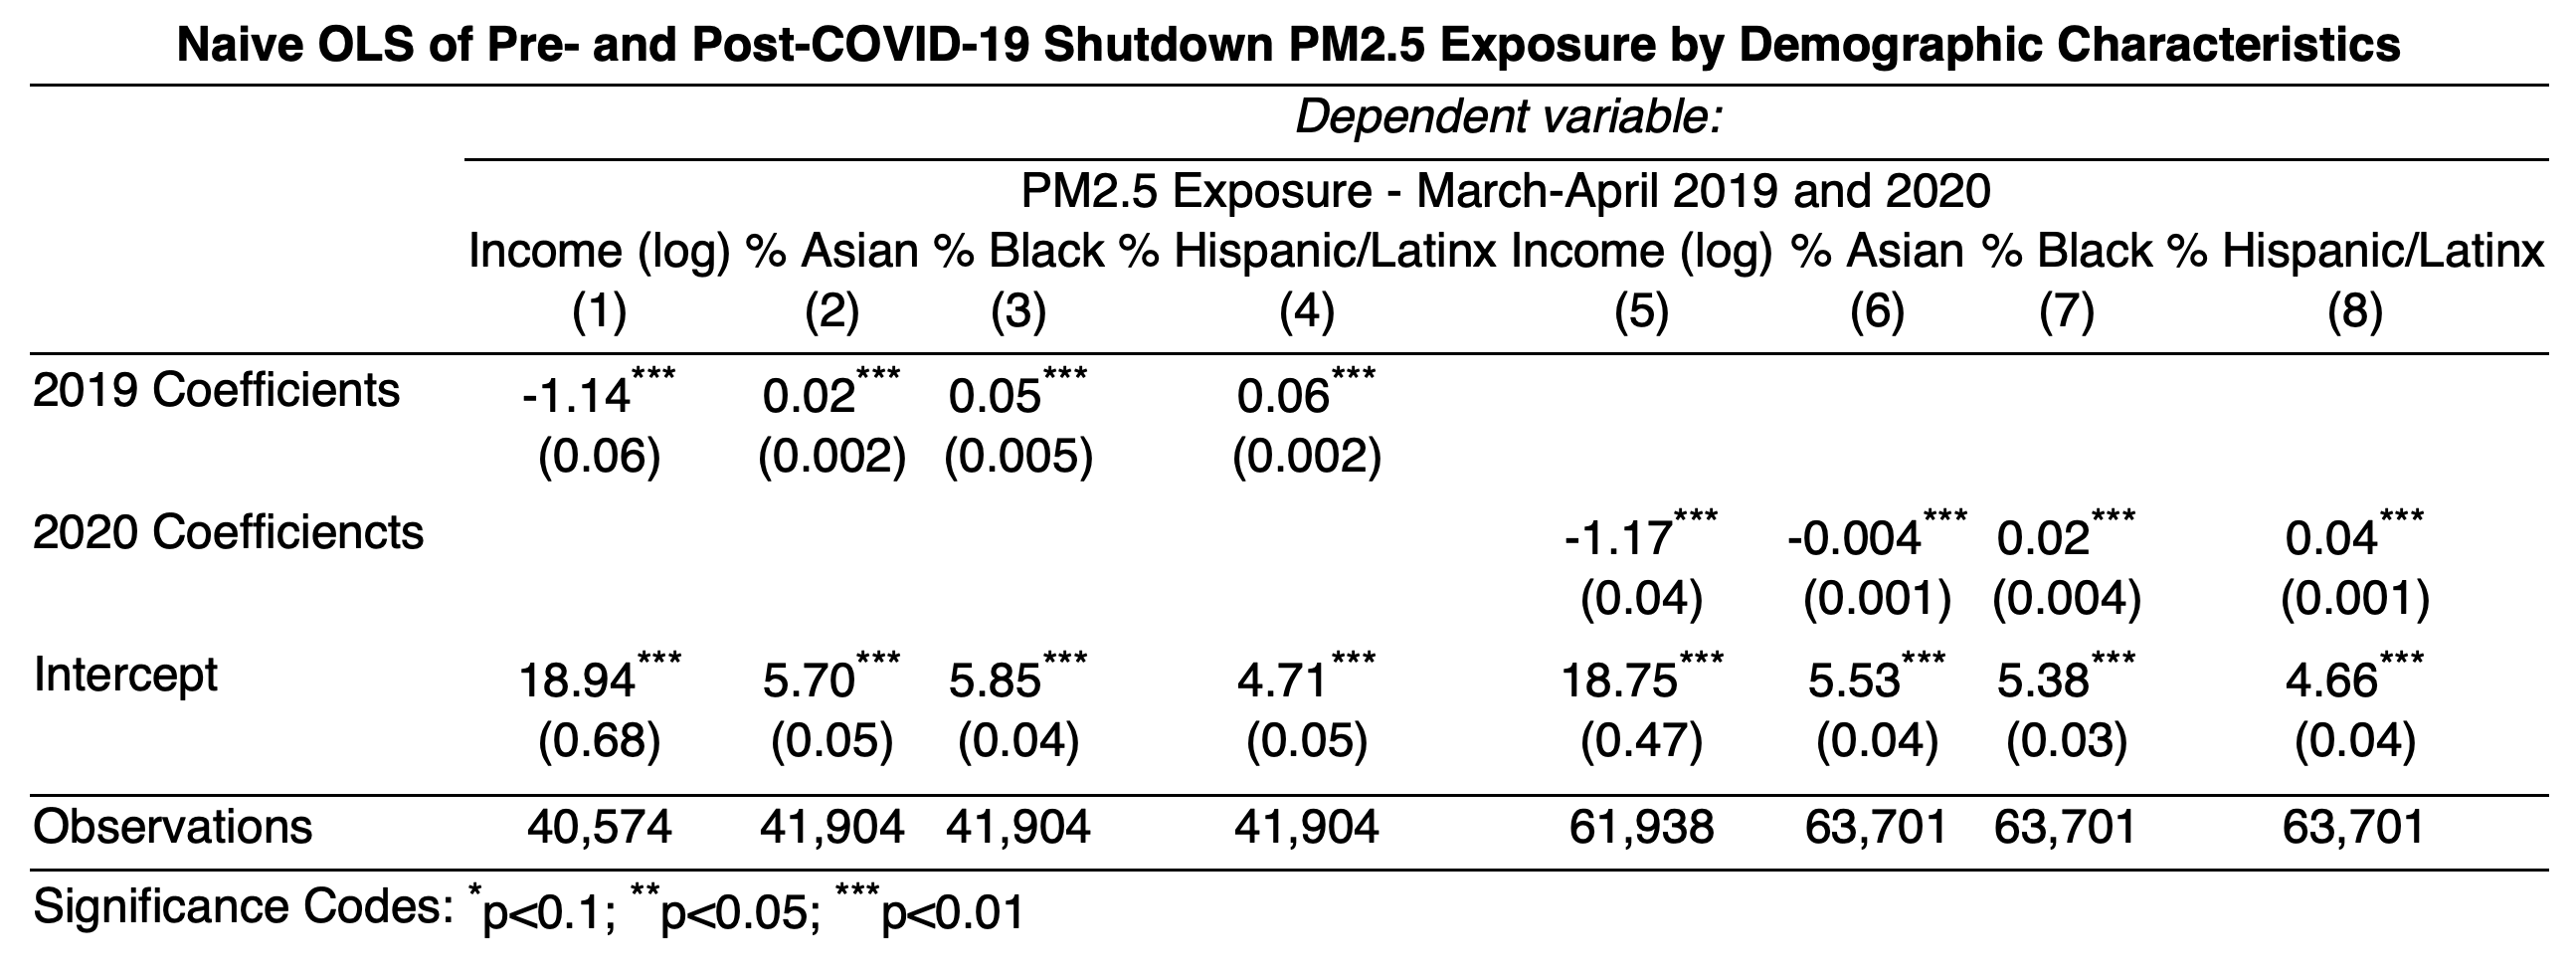
\includegraphics{figures/PM_fits_white.png}

}

\caption{\label{fig-reg-table}Summary table of regressions grouped by
year and demographic characteristics including percent compositions of
racial groups and income.}

\end{figure}

\newpage

\hypertarget{conclusion}{%
\section{Conclusion}\label{conclusion}}

The findings of this paper largely confirm previous studies in the
field, particularly in terms of the discrepancies in particulate matter
exposure between different racial and income groups. County-level
analyses were mixed but found a small reduction in average exposure
across the entire sampled population. When broken down by racial groups,
there was a noticeable reduction in PM2.5 exposure among all groups,
although the largest reductions were seen Black and some Hispanic/Latinx
communities. This analysis demonstrates an important overarching dynamic
at the heart of environmental justice scholarship. However, it also
highlights the importance of continued study into what factors may
contribute to and confound an understanding of air pollution exposure
over various spatial and temporal scales.

\hypertarget{refs}{}

\begin{CSLReferences}{0}{0}\end{CSLReferences}

\appendix

\hypertarget{appendix}{%
\section{Appendix}\label{appendix}}

All scripts and files needed to replicate this paper are stored across
two locations and can be downloaded from the following repositories:

\url{https://github.com/andreeanes/aqrd-final} (main repository)

\url{https://drive.google.com/drive/folders/1e0YykCVAuH_S8EYyPQWqV3jU1sGu_HYT?usp=sharing}
(larger datasets \texttt{PM.csv} and \texttt{PMlong\_bins\_all.csv},
which should be saved into the main repository's \texttt{data} folder)

The entire original replication package for
\citet{bluhm_disparate_2022}, including raw datasets and the code which
creates the data frames used for this analysis, is stored across two
locations. The main repository containing code, figures, and smaller
datasets can be downloaded at
\href{https://github.com/jaburney/CA-COVIDEJ-2022/tree/main}{https://github.com/jaburney/CA-COVIDEJ-2022},
while the Dataverse where the largest datasets can be downloaded is
located at \url{https://doi.org/10.7910/DVN/ZXVB7A}

% END BODY %%%%%%%%%%%%%%%%%%%%%%%%%%%%%%%%%%%%%%%%%%%%%%%%%%%%%%%%%%%%%%%%%%%%%



\end{document}
